\documentclass [12pt]{article}
\usepackage{graphicx}

\title{{\Huge \textbf{Dodgeball Tactics}}}
\author{Zach Stecher}
\date{Due: 9/22/16}

\begin{document}


\maketitle
\newpage

\section*{Game Overview}
Dodgeball Tactics is a turn-based tactical game set in the gym of your neighborhood school. As the school's new dodgeball coach, you are charged with turning your small town group of rag tags into a team worthy of winning the national championship. You will utilize strategic thinking to ensure your players are put in the best possible situation to win!

All the chaos of dodgeball is distilled down to a chess-like match of positioning and formation where the team with the superior gameplan will come out on top. Building your team to suit your playstyle and deploying your players correctly will be crucial to claiming your place at the top of the dodgeball pyramid! Once you've established yourself, take your skills to the exhibition circuit and challenge your friend to a head-to-head matchup to find out who's the better coach!

Lead your team against the computer or another player and make use of positioning and strategy to eliminate the other team before they get you out first! Get close for better aim or farther away to make it more difficult for the other team. Above all, remember the 5 D's: Dodge, Duck, Dip, Dive and Dodge!

Dodgeball tactics is intended for players age 12 and up who enjoy competitive tactical games and will launch on the PC platform. Players will have to think ahead and plan their attacks and defensive maneuvers in order to maximize their team's abilities and end up on top. The game is designed to provide a strategic challenge and make players think and consider multiple different avenues to victory while conveying the sense of chaos that dodgeball games are synonymous with. By combining a tactical, turn-based design with an element of randomness, Dodgeball Tactics becomes a product that is easy to learn, but difficult to master.

There are an incredible amount of lineup, positioning and strategic combintions that give Dodgeball Tactics a phenomenal level of replayability. There's no one correct way to win an individual game!
\newpage

\section*{Feature List}

\begin{itemize}
\item Employ a near-infinite number of possible tactics to overwhelm or outsmart your opponent!
	\begin{itemize}
	\item With a grid based board and the ability to move your units in any direction, the possibilities are nearly endless!
	\end{itemize}

\item Build your team from the ground up!
	\begin{itemize}
	\item Start with a small team and recruit more players as you go. Stack your bench with extra players!
	\end{itemize}

\item Pick your starting lineup from a selection of different players. Start the team that fits your coaching style!
	\begin{itemize}
	\item Mix and match your unit types and their starting positions for each match. If one lineup doesn't work, try a different one!
	\end{itemize}

\item Play against your friends!
	\begin{itemize}
	\item Go head to head with a friend for dodgeball dominance! Players can initiate local multiplayer games and match their coaching prowess against another player for infinite replayability!
	\end{itemize}

\item Knock out opposing players by hitting them with dodgeballs or catching dodgeballs thrown at you!
	\begin{itemize}
	\item Successfully hit an opposing player to eliminate them, or get lucky and catch a ball thrown at you to eliminate the player that threw it, AND get one of your eliminated players back!
	\end{itemize}

\item Position your players carefully!
	\begin{itemize}
	\item Players are harder to hit with someone standing in front of them. Guard your important players carefully and don't let the opponent isolate key players!
	\end{itemize}

\item You choose the overall gameplan!
	\begin{itemize}
	\item Stockpile balls to let loose a single turn barrage or keep up the constant pressure to force your opponents back. The decision is up to you!
	\end{itemize}

\item Play as the Ace!
	\begin{itemize}
	\item Every team has that one player who's simply better than everyone else playing. Well, your team has one too! Use him correctly and he could have a huge impact on the game!
	\end{itemize}

\item Eliminate every player on the other team to win!
	\begin{itemize}
	\item Show no mercy! Even one leftover player has the power to change the flow of a game.
	\end{itemize}

\end{itemize}

\section*{Development Estimate}

\subsection*{Time Estimate}

Dodgeball Tactics should take no longer than 3 months from beginning of development to initial launch. Beginning of development is classified as the start of asset procurement/creation or progamming. The game system and mechanics will need to be programmed and confirmed to work first, in concert with obtaining and implementing art assets. QA will likely encompass the final third of development at minimum in order to ensure all systems work together correctly.

\subsection*{Budget}

\begin{itemize}
\item \$20,750 for programmer salary.
\item \$22,000 for producer/programmer salary.
\item \$15,000 for miscellaneous expenses. Audio and art assets will be obtained from a freelance source on a per asset basis.
\end{itemize}
\newpage

\section*{Competitive Analysis}

Dodgeball Tactics seeks to enter a currently slumping turn-based tactical game market. While the genre was surging fairly recently with titles like Final Fantasy Tactics, Advance Wars, and XCOM, the current landscape is mostly older re-releases or titles under the similar but more multitasking, twitch based Real Time Strategy genre. Dodgeball Tactics looks to capitalize on the current lull in turn based strategy titles, while also offering up a different experience.

Most turn based strategy games provide a war-based background where players do battle with soldiers, tanks, swords, or other weapons. These units also usually come with a plethora of different abilities. While this provides for a high level of tactical planning and thinking, the sheer amount of variables present can be overwhelming for newer players and lead them to simply choose the most straightforward way of completing a given level, or just give up and stop playing entirely!

In contrast, Dodgeball Tactics seeks to provide a fun, compact version of these games that allows for a medium to high level of strategic thinking without forcing the player to learn dozens of different abilities and unit traits in order to make informed choices and be successful. Players should be able to pick up the game within a few minutes and start having fun.

Warhammer and Warhammer 40,000 provide the largest inspirations for Dodgeball Tactics, but require a large investment by the player to purchase the miniatures, paint them, and learn the complicated rules. If a player wishes to change his or her army, they must make the same investment again. Dodgeball Tactics wants to tap into the strategy that keeps players returning to Warhammer, but without the large up-front investment and barrier to entry.

Many of these games also rely on map differences to provide a challenge. Each level will have a different layout with different "traps" or "hazards", along with varying enemy unit placement. This provides excitement with a high level of unknown factors to account for while playing, however this can also cause a lot of player frustration when they encounter a detrimental effect with no warning. Players may feel cheated by the game system if they lose due to something like this. This method of providing challenge also often means that levels are static, and multiple playthroughs will result in players memorizing the locations of these effects. This allows players to determine an optimal playthrough that will stay the same every time you replay a level, resulting in low replayability.

Dodgeball Tactics seeks to provide a high amount of replayability by offering players the ability to play against each other. Similar to games like Chess and Warhammer, Dodgeball Tactics is intended to provide an environment where no two games will play out exactly the same, but in a digital form. In the end, Dodgeball Tactics is a game designed to be played by two players against each other.

\section*{Expansion Plans}

\begin{itemize}
\item Challenge Mode
	\begin{itemize}
	\item Win games with extra rules or restrictions such as a limit on units, turn limit, or other disadvantages.
	\end{itemize}

\item Online Features
	\begin{itemize}
	\item Online multiplayer to enable players to match up against each other from their own homes.
	\end{itemize}
	\begin{itemize}
	\item Skill levels and leaderboards to allow players to know who the best coach around is.
	\end{itemize}
	\begin{itemize}
	\item Organized tournaments. The actual nationals!
	\end{itemize}

\item Upgrade your gym!
	\begin{itemize}
	\item New art for your team's home gym background. Obtained either through DLC purchase, or earned from tournaments or high leaderboard results, your school team should be able to show its pride! Playing in the school gym may be the tried and true way, but who wouldn't want their gym to be in space?
	\end{itemize}

\item New team uniforms
	\begin{itemize}
	\item And not just the shirts. Assemble a team of demons or tigers to replace the frail children you used to coach!
	\end{itemize}
\end{itemize}

\section*{Concept Art}

\begin{figure}[!htb]
	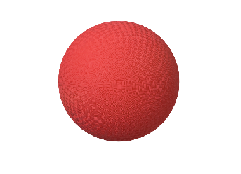
\includegraphics{dodgeball.png}
	\caption{A dodgeball.}
\end{figure}

\begin{figure}[!htb]
	
\includegraphics{player.png}
	\caption{Player Concept.}
\end{figure}

\begin{figure}[!htb]
	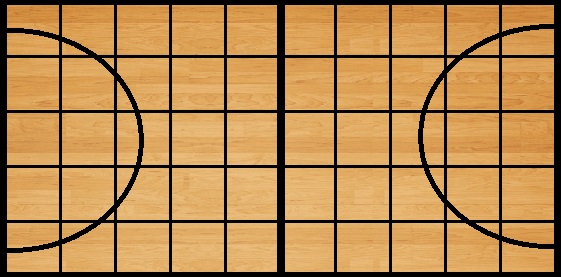
\includegraphics{DBT_Background.png}
	\caption{Court Concept.}
\end{figure}

\end{document}